\documentclass[12pt]{article}
\usepackage[utf8]{inputenc}
\usepackage[spanish]{babel}
\usepackage{amsmath}
\usepackage{amsthm}
\usepackage{hyperref}
\usepackage{graphicx}
\usepackage{color}
\usepackage{float}
\usepackage{multicol}
\usepackage{enumerate}
\usepackage{anyfontsize}
\usepackage{anysize}
\usepackage{tikz}
\usepackage{siunitx}
\usepackage{gensymb}
\usetikzlibrary{arrows.meta, positioning}
\setlength{\parskip}{1em}
\spanishdecimal{.}


\title{Ejercicios de repaso \vspace{-2cm}}
\author{}
\date{ }

%--------------------------------------------------------------------
\newcounter{choice}
\renewcommand\thechoice{\Alph{choice})}
%\newcommand\choicelabel{\thechoice.}
\newcommand\choicelabel{\thechoice}

\newenvironment{choices}%
  {\list{\choicelabel}%
     {\usecounter{choice}\def\makelabel##1{\hss\llap{##1}}%
       \settowidth{\leftmargin}{W.\hskip\labelsep\hskip 2.5em}%
       \def\choice{%
         \item
       } % choice
       \labelwidth\leftmargin\advance\labelwidth-\labelsep
       \topsep=0pt
       \partopsep=0pt
     }%
  }%
  {\endlist}

\newenvironment{oneparchoices}%
  {%
    \setcounter{choice}{0}%
    \def\choice{%
      \refstepcounter{choice}%
      \ifnum\value{choice}>1\relax
        \penalty -50\hskip 1em plus 1em\relax
      \fi
      \choicelabel
      \nobreak\enskip
    }% choice
    % If we're continuing the paragraph containing the question,
    % then leave a bit of space before the first choice:
    \ifvmode\else\enskip\fi
    \ignorespaces
  }%
  {}
%----------------------------------------------------------

\begin{document}
\maketitle
\fontsize{14}{14}\selectfont

Escribe las parejas de ángulos que se piden.
\begin{figure}[H]
    \centering
    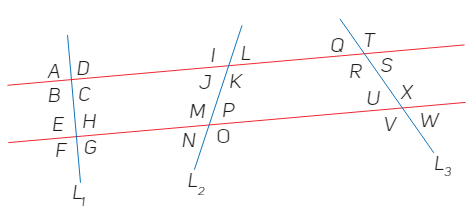
\includegraphics[scale=1]{Imagenes/Angulos_04.png}
\end{figure}
\begin{enumerate}[label=\alph*)]
\item Parejas de ángulos correspondientes formados con la transversal $L_{1}$ 
\\  \textbf{R. } \rule{2cm}{0.1mm}
\item Parejas de ángulos colaterales internos formados con la transversal $L_{2}$ 
\\  \textbf{R. } \rule{2cm}{0.1mm}
\item Parejas de ángulos colaterales externos formados con la transversal $L_{2}$ 
\\  \textbf{R. } \rule{2cm}{0.1mm}
\item Parejas de ángulos alternos internos formados con la transversal $L_{3}$ 
\\  \textbf{R. } \rule{2cm}{0.1mm}
\item Parejas de ángulos alternos externos formados con la transversal $L_{3}$ 
\\  \textbf{R. } \rule{2cm}{0.1mm}
\end{enumerate}

\newpage

En una figura formada por dos rectas parelaleas cortadas por una transversal:
\begin{itemize}
\item Los ángulos correspondientes miden los mismo.
\item Los ángulos alternos internos miden lo mismo.
\item Los ángulos alternos externos miden lo mismo.
\end{itemize}

En la siguiente figua, las rectas son paralelas. Determina la medida de los ángulos marcados con letras.
\begin{figure}[H]
    \centering
    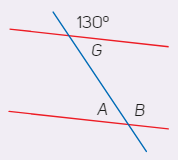
\includegraphics[scale=1.25]{Imagenes/Angulos_05.png}
\end{figure}
$\measuredangle \, A =$ \rule{2cm}{0.1mm} \hspace{0.4cm} $\measuredangle \, B =$ \rule{2cm}{0.1mm} \hspace{0.4cm} $\measuredangle \, G =$ \rule{2cm}{0.1mm}
\end{document}